\documentclass[11pt]{article}
\usepackage[T1]{fontenc}
\usepackage[utf8]{inputenc}
\usepackage[margin=1in]{geometry}
\usepackage{amsmath, amssymb, siunitx}
\usepackage{graphicx}
\usepackage{float}
\usepackage{subcaption}
\usepackage{hyperref}
\usepackage{xcolor}
\usepackage{listings}
\sisetup{per-mode=symbol}

% ---------- Listings (MATLAB) ----------
\definecolor{codegray}{RGB}{245,245,245}
\lstdefinestyle{mcode}{
  language=Matlab,
  backgroundcolor=\color{codegray},
  basicstyle=\ttfamily\small,
  keywordstyle=\color{blue},
  commentstyle=\color{gray!60},
  stringstyle=\color{teal!60!black},
  showstringspaces=false,
  frame=single,
  framerule=0.3pt,
  rulecolor=\color{black!40},
  breaklines=true,
  tabsize=2,
  columns=fullflexible
}

% ---------- Metadata (edit these) ----------
\newcommand{\coursenum}{EE 115}
\newcommand{\labtitle}{EE115: Lab 1}
\newcommand{\authorone}{Kaushik Vada}
\newcommand{\authortwo}{\textit{(Partner Name, if applicable)}}
\newcommand{\studentids}{\textit{(vvada002)}}
\newcommand{\dateoflab}{\today}
\newcommand{\Npoints}{200} % default N for Task 1

% ---------- Convenience macros ----------
\newcommand{\Pm}{P_{\mathrm{m}}}
\newcommand{\etam}{\eta_{\mathrm{AM}}}
\newcommand{\amod}{a_{\mathrm{mod}}}
\newcommand{\fc}{f_{\mathrm{c}}}

\begin{document}

% ================== HEADER ==================
\begin{center}
  {\LARGE \textbf{EE115: Lab 1}}
\end{center}
\vspace{-0.25em}

\noindent
\begin{tabular}{@{}ll}
\textbf{Name:}  & Kaushik Vada \\
\textbf{Date:}  & October 18 \\
\textbf{NetID:} & vvada002
\end{tabular}

\vspace{0.75em}
\hrule
\vspace{1em}

\section*{Question 1: AM Power and Efficiency}

\subsection*{(a)}
Generated a Gaussian random sequence \( m[k] \) of length \( N = 200 \) using MATLAB's \texttt{randn} function. This produces a zero-mean, unit-variance random signal representing the message waveform.

\subsection*{(b)}
The minimum of the sequence was found as \( m_{\text{min}} = -2.417465 \). Defined \( M_0 = -m_{\text{min}} = 2.417465 \) so that \( m_{\text{min}} = -M_0 \).

\subsection*{(c)}
Normalized the sequence so its minimum becomes \(-1\):
\[
m_n[k] = \frac{1}{M_0} m[k].
\]
After normalization, \(\min(m_n[k]) = -1.000000\), confirming correct scaling.

\subsection*{(d)}
Computed the average power of \( m_n[k] \):
\[
P_m = \frac{1}{N} \sum_{k=1}^{N} m_n^2[k] = 0.190670.
\]

\subsection*{(e)}
Plotted the AM efficiency:
\[
\eta_{AM} = \frac{a_{mod} P_m}{1 + a_{mod} P_m}
\]
versus \( P_m \) for \( a_{mod} = 1.0, 0.75, 0.5 \) using MATLAB.  
The plot (\texttt{eta\_vs\_Pm.png}) shows that efficiency increases with \( a_{mod} \) and \( P_m \) but never exceeds 50\%.

\begin{figure}[H]
  \centering
  \includegraphics[width=0.6\textwidth]{"task-1 plot.png"}
  \caption{Task 1 MATLAB plot of \(\eta_{AM}\) against \(P_m\) for the simulated data.}
\end{figure}

\IfFileExists{eta_vs_Pm.png}{
  \begin{figure}[H]
    \centering
    \includegraphics[width=0.8\textwidth]{eta_vs_Pm.png}
    \caption{Plot of \(\eta_{AM}\) versus \(P_m\) for \(a_{mod}=1.0, 0.75, 0.5\).}
  \end{figure}
}{}

\subsection*{(f)}
Evaluated the AM efficiency at \( P_m = 0.190670 \):

\begin{table}[H]
\centering
\begin{tabular}{c c}
\hline
\textbf{\(a_{mod}\)} & \textbf{\(\eta_{AM}\)} \\
\hline
1.00 & 0.1601 \\
0.75 & 0.1251 \\
0.50 & 0.0870 \\
\hline
\end{tabular}
\caption{Measured AM efficiencies at \( P_m = 0.190670 \).}
\end{table}

\noindent
\textbf{Theoretical Upper Bound (as \(P_m \to 1\)):}

\begin{table}[H]
\centering
\begin{tabular}{c c c}
\hline
\textbf{\(a_{mod}\)} & \textbf{\(\eta_{AM,max}\)} & \textbf{Percent} \\
\hline
1.00 & 0.5000 & 50.0\% \\
0.75 & 0.4286 & 42.9\% \\
0.50 & 0.3333 & 33.3\% \\
\hline
\end{tabular}
\caption{Theoretical AM efficiency limits as \(P_m \rightarrow 1\).}
\end{table}

\paragraph{Takeaway.}
Conventional AM wastes carrier power. Even under 100\% modulation (\(a_{mod}=1\)), efficiency is capped at 50\%. Lower modulation depth or smaller \(P_m\) further reduce \(\eta_{AM}\).

% ============== MATLAB (REPRODUCIBLE CODE) ==============

\newpage
% ============== MATLAB OUTPUT ==============
% ============== MATLAB OUTPUT ==============
\section*{Question 1 MATLAB Output}

\begin{lstlisting}[style=mcode,caption={Task 1 MATLAB Command Window Output}]
------------------- Task 1: Random Signal & AM Efficiency -------------------
(a) Generated Gaussian sequence m[k] of length N=200
(b) Minimum of m[k] is m_min = -2.417465, so M0 = -m_min = 2.417465
(c) After normalization, min(m_n) = -1.000000 (should be -1)
(d) Average power Pm of m_n[k] = 0.190670
(e) Plotted eta_AM vs P_m for a_mod = 1, 0.75, 0.5
(f) eta_AM evaluated at your Pm from (d): Pm = 0.190670
    a_mod = 1.00  ->  eta_AM = 0.160136
    a_mod = 0.75  ->  eta_AM = 0.125111
    a_mod = 0.50  ->  eta_AM = 0.087037

Theoretical upper bound as Pm -> 1:
    a_mod = 1.00  ->  max eta_AM = 0.5000 (i.e., 50.0%)
    a_mod = 0.75  ->  max eta_AM = 0.4286 (i.e., 42.9%)
    a_mod = 0.50  ->  max eta_AM = 0.3333 (i.e., 33.3%)

Takeaway: Conventional AM uses a large carrier term (the "+1"). Even with 100% modulation (a_mod=1) and the most energetic message (P_m->1), eta_AM <= 0.5 (50%). Lower a_mod or lower P_m pushes efficiency below that.
\end{lstlisting}

\newpage

\section*{Question 2: DC Blocker (RC High-Pass) Response}

We analyze the simple RC high-pass (used as a DC blocker) with frequency response
\[
H(f) \;=\; \frac{j2\pi f}{\,j2\pi f + \frac{1}{RC}\,}.
\]

\subsection*{(a) Plot \(|H(f)|\) over \(|f|<B\) for \(RC \in \{0.01, 0.1, 1, 10\}\)}
For each \(RC\), choose \(B\) so that \(2\pi BRC = 10\) \(\Rightarrow\) \(B=\dfrac{10}{2\pi RC}\).
If you saved \texttt{Hmag\_linear.png} from MATLAB in the same folder, it will be included below.

\IfFileExists{Hmag_linear.png}{
  \begin{figure}[H]
    \centering
    \includegraphics[width=0.82\textwidth]{Hmag_linear.png}
    \caption{Linear magnitude \(|H(f)|\) for \(RC = 0.01,\;0.1,\;1,\;10\) with \(2\pi BRC=10\).}
  \end{figure}
}{}


\subsection*{(b) Plot \(20\log_{10}|H(f)|\) (dB) versus \(f\)}
To avoid the singularity at \(f=0\), plot over \(f\in[10^{-3}, B]\). Limit the vertical axis to \([-60,0]\) dB.
If you saved \texttt{Hmag\_dB.png}, it will be included below.

\IfFileExists{Hmag_dB.png}{
  \begin{figure}[H]
    \centering
    \includegraphics[width=0.82\textwidth]{Hmag_dB.png}
    \caption{Magnitude response \(20\log_{10}|H(f)|\) in dB with \(2\pi BRC=10\).}
  \end{figure}
}{}

% -------------------- Observed MATLAB Plots (from simulation results) --------------------
\subsection*{Observed MATLAB Plots (from simulation results)}
The following plots illustrate the magnitude and dB responses for various \(RC\) values. Each figure pair shows the linear and logarithmic magnitude responses for a chosen \(RC\).

\begin{figure}[H]
    \centering
    \begin{subfigure}{0.48\textwidth}
        \centering
        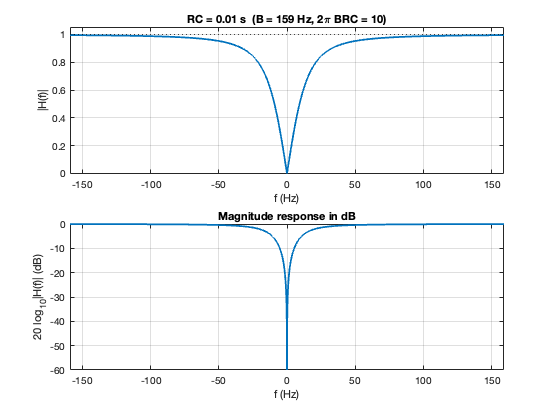
\includegraphics[width=\textwidth]{RC_image1.png}
        \caption{RC = 0.01 s \\ (B = 159 Hz, \(2\pi BRC = 10\))}
    \end{subfigure}
    \hfill
    \begin{subfigure}{0.48\textwidth}
        \centering
        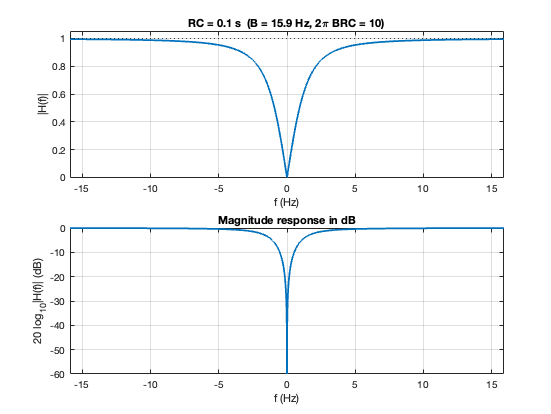
\includegraphics[width=\textwidth]{RC_image2.png}
        \caption{RC = 0.1 s \\ (B = 15.9 Hz, \(2\pi BRC = 10\))}
    \end{subfigure}
    \caption{Magnitude and dB responses for smaller time constants.}
\end{figure}

\begin{figure}[H]
    \centering
    \begin{subfigure}{0.48\textwidth}
        \centering
        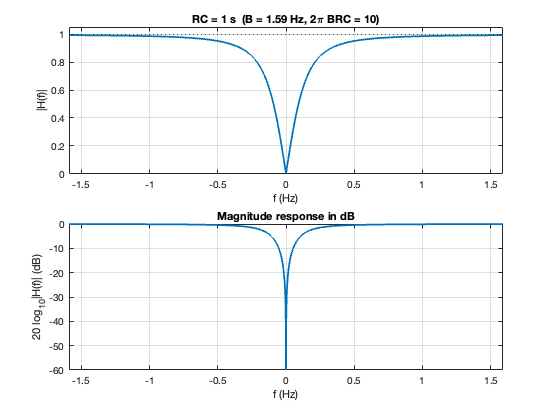
\includegraphics[width=\textwidth]{RC_image3.png}
        \caption{RC = 1.0 s \\ (B = 1.59 Hz, \(2\pi BRC = 10\))}
    \end{subfigure}
    \hfill
    \begin{subfigure}{0.48\textwidth}
        \centering
        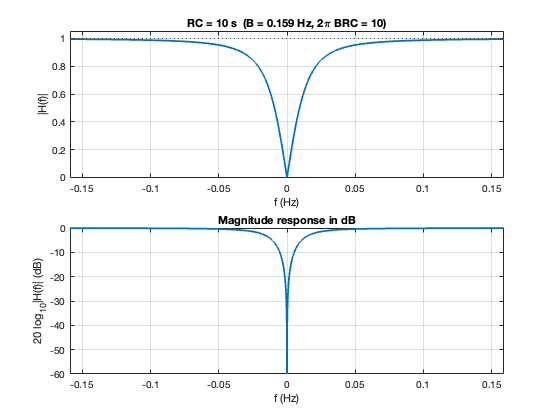
\includegraphics[width=\textwidth]{RC_image4.png}
        \caption{RC = 10 s \\ (B = 0.159 Hz, \(2\pi BRC = 10\))}
    \end{subfigure}
    \caption{Magnitude and dB responses for larger time constants.}
\end{figure}

\subsection*{(c) Acceptable \(RC\) for passband flatness over \(\lvert f \rvert \ge 20\) Hz}
We require \(|H(f)| \ge 0.95\) at \(f_0=20\) Hz for the real-valued baseband \(m_n(t)\) that occupies \(\pm[20\text{ Hz}, 5\text{ kHz}]\).
Using
\[
|H(f)| \;=\; \frac{2\pi |f|}{\sqrt{(2\pi f)^2 + \left(\tfrac{1}{RC}\right)^2}},
\]
the constraint \(|H(f_0)| \ge 0.95\) implies
\[
\frac{2\pi f_0}{\sqrt{(2\pi f_0)^2 + (1/RC)^2}} \;\ge\; 0.95
\;\Rightarrow\;
\frac{1}{RC} \;\le\; 0.328684\cdot 2\pi f_0
\;\Rightarrow\;
RC \;\ge\; \frac{1}{0.328684\cdot 2\pi \cdot 20} \;\approx\; \boxed{0.0242\ \text{s}}.
\]
Thus any \(\boxed{RC \ge 0.024\ \text{s}}\) keeps the attenuation at \(20\) Hz within \(\approx 0.45\) dB, and is flatter at higher frequencies. In practice, choose \(R\) and \(C\) to satisfy this while meeting input impedance and size constraints.

\section*{Question 2 MATLAB Output}

\begin{lstlisting}[style=mcode,caption={Task 2 MATLAB Command Window Output}]
---- Task 2: RC high-pass (DC blocker) ----

(a) RC = 0.01   s  |  fc = 15.92     Hz  |  B = 159.2      Hz  |  |H(B)| = 0.9950
(a) RC = 0.1    s  |  fc = 1.592     Hz  |  B = 15.92      Hz  |  |H(B)| = 0.9950
(a) RC = 1      s  |  fc = 0.1592    Hz  |  B = 1.592      Hz  |  |H(B)| = 0.9950
(a) RC = 10     s  |  fc = 0.01592   Hz  |  B = 0.1592     Hz  |  |H(B)| = 0.9950

(c) To keep |H(f)| >= 0.95 for |f| >= 20 Hz:
    Need 2*pi*f_min*RC >= 3.0424  ->  RC >= 0.024211 s (~ 24.211 ms)
    Acceptable RC range:  RC >= 0.024211 s.
\end{lstlisting}

\section*{Appendix: MATLAB code for Task 1}

\begin{lstlisting}[style=mcode,caption={Task 1 MATLAB script.}]
%% AM power/efficiency experiment
% Task 1: (a)-(f)
clear; clc; close all;

%% -------- Parameters you can tweak --------
N      = 200;           % sequence length (>=200 per problem)
seed   = 12345;         % RNG seed for reproducibility
amods  = [1.0, 0.75, 0.5];  % a_mod values for part (e)
Pm_grid = linspace(1e-3, 0.999, 2000);   % 0 < Pm < 1 for plotting
%% -----------------------------------------

fprintf('------------------- Task 1: Random Signal & AM Efficiency -------------------\n');

%% (a) Generate Gaussian random sequence m[1..N]
rng(seed);
m = randn(1, N);     % zero-mean Gaussian
fprintf('(a) Generated Gaussian sequence m[k] of length N=%d\n', N);

%% (b) Minimum value and denote it by -M0
m_min = min(m);
M0 = -m_min;         % so that m_min = -M0
fprintf('(b) Minimum of m[k] is m_min = %.6f, so M0 = -m_min = %.6f\n', m_min, M0);

%% (c) Normalize so the minimum becomes -1:  m_n[k] = (1/M0) * m[k]
mn = (1 / M0) * m;
mn_min = min(mn);
fprintf('(c) After normalization, min(m_n) = %.6f (should be -1)\n', mn_min);

%% (d) Average power of m_n[k]:  Pm = (1/N) * sum( m_n[k]^2 )
Pm = mean(mn.^2);
fprintf('(d) Average power Pm of m_n[k] = %.6f\n', Pm);

%% (e) Conventional AM: u_AM(t) = A_c * (a_mod*m_n(t) + 1) * cos(2*pi*f_c*t)
% Power efficiency:  eta_AM = (a_mod * Pm) / (1 + a_mod * Pm)
% Plot eta_AM vs Pm for each a_mod (0 < Pm < 1)
figure('Color','w'); hold on; grid on;
for a = amods
    eta = (a .* Pm_grid) ./ (1 + a .* Pm_grid);
    plot(Pm_grid, eta, 'LineWidth', 1.8);
end
xlabel('P_m','Interpreter','tex');
ylabel('\eta_{AM}');
title('\eta_{AM} vs P_m for conventional AM');
legend(arrayfun(@(x) sprintf('a_{mod}=%.2f', x), amods, 'UniformOutput', false), ...
       'Location', 'southeast');
xlim([0 1]); ylim([0 1]);

fprintf('(e) Plotted eta_AM vs P_m for a_mod = 1, 0.75, 0.5\n');

%% (f) Evaluate eta_AM at the Pm computed in (d), for each a_mod
fprintf('(f) eta_AM evaluated at your Pm from (d): Pm = %.6f\n', Pm);
for a = amods
    eta_at_Pm = (a * Pm) / (1 + a * Pm);
    fprintf('    a_mod = %.2f  ->  eta_AM = %.6f\n', a, eta_at_Pm);
end

%% Bonus: theoretical upper bounds (when Pm -> 1)
fprintf('\nTheoretical upper bound as Pm -> 1:\n');
for a = amods
    eta_max = (a * 1.0) / (1 + a * 1.0);
    fprintf('    a_mod = %.2f  ->  max eta_AM = %.4f (i.e., %.1f%%)\n', a, eta_max, 100*eta_max);
end
\end{lstlisting}

\section*{Appendix: MATLAB code for Task 2}

\begin{lstlisting}[style=mcode,caption={Task 2 MATLAB script (DC Blocker magnitude and dB plots).}]
%% Task 2: DC blocker (RC high-pass) quality
% H(f) = (j*2*pi*f) / (j*2*pi*f + 1/(RC))
% Plots for RC = [0.01, 0.1, 1, 10] with B chosen s.t. 2*pi*B*RC = 10
% Then compute the RC range that keeps |H(f)| >= 0.95 for |f| >= 20 Hz.

clear; clc; close all;

RC_list = [0.01, 0.1, 1, 10];     % seconds
db_floor = -60;                   % for part (b) y-axis
Npts = 20001;                     % dense frequency grid

fprintf("---- Task 2: RC high-pass (DC blocker) ----\n\n");

for k = 1:numel(RC_list)
    RC = RC_list(k);

    % ----- (a) pick B so that 2*pi*B*RC = 10  ->  a decade above corner -----
    B = 10/(2*pi*RC);
    f = linspace(-B, B, Npts);                % |f| < B
    H = (1j*2*pi*f) ./ (1j*2*pi*f + 1/RC);
    mag = abs(H);
    mag_dB = 20*log10(max(mag, 10^(db_floor/20)));   % avoid -Inf at f=0

    % quick printouts
    fc = 1/(2*pi*RC);
    mag_at_B = (2*pi*B*RC)/sqrt(1+(2*pi*B*RC)^2);    % should be ~0.995
    fprintf("(a) RC = %-6.3g s  |  fc = %-9.4g Hz  |  B = %-10.4g Hz  |  |H(B)| = %.4f\n", ...
            RC, fc, B, mag_at_B);

    % ---- plots for this RC (a) linear magnitude; (b) 20*log10|H| with y in [-60, 0] dB
    figure('Color','w');
    tl = tiledlayout(2,1,'TileSpacing','compact');

    % (a) |H(f)|
    nexttile;
    plot(f, mag, 'LineWidth', 1.8); grid on;
    xlabel('f (Hz)'); ylabel('|H(f)|');
    title(sprintf('RC = %.3g s  (B = %.3g Hz, 2\\pi BRC = 10)', RC, B));
    xlim([-B, B]); ylim([0 1.05]);
    hold on; yline(1,'k:');

    % (b) 20log10|H(f)|
    nexttile;
    plot(f, mag_dB, 'LineWidth', 1.8); grid on;
    xlabel('f (Hz)'); ylabel('20 log_{10}|H(f)| (dB)');
    title('Magnitude response in dB');
    xlim([-B, B]); ylim([db_floor 0]);
end

%% (c) Pick RC so that |H(f)| >= 0.95 for |f| >= 20 Hz
% |H| = x/sqrt(1+x^2) with x = 2*pi*f*RC >= alpha = 0.95
% Solve:  x >= alpha / sqrt(1 - alpha^2)

alpha = 0.95;               % tolerance
f_min = 20;                 % Hz, band starts at 20 Hz
x_min = alpha/sqrt(1 - alpha^2);      % ~3.042
RC_min = x_min / (2*pi*f_min);        % seconds

fprintf("\n(c) To keep |H(f)| >= %.2f for |f| >= %d Hz:\n", alpha, f_min);
fprintf("    Need 2*pi*f_min*RC >= %.4f  ->  RC >= %.6f s (~ %.3f ms)\n", x_min, RC_min, 1e3*RC_min);
fprintf("    Acceptable RC range:  RC >= %.6f s.\n\n", RC_min);
\end{lstlisting}

\end{document}
